\section{Referentni podaci}

Referentni podaci su oni podaci s kojima se uspoređuju rezultati metoda. Ti referentni podaci su generirani u simulatoru te predstavljaju lokaciju i rotaciju vozila u jednome trenutku. Referentni podaci se zapravo sastoje od lokacije i rotacije vozila.

\subsubsection{Lokacija}
Lokacija vozila je također definirana kao točka u kartezijevom koordinatnome prostoru. Sastoji se od x, y i z koordinata. Slično kao prikazano na slici \ref{fig:point_coordinates}.


\subsubsection{Rotacija}
 U trodimenzialnome prostoru objekt se zapravo može rotirati oko beskonaćnoga broja osi ali se u pravilu uzimaju 3 statičke osi. Te osi se nazivaju os skretanja (eng. yaw), os poniranja (eng. pitch) i os valjanja (eng. roll). 

\begin{figure}[ht!]
  \centering
  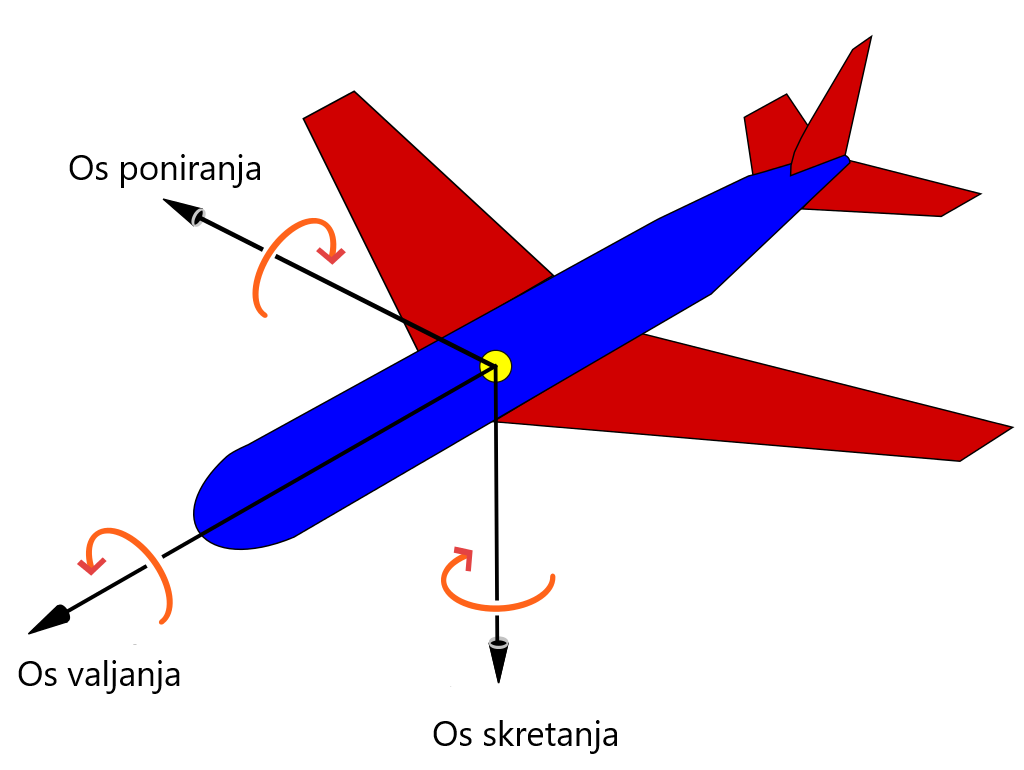
\includegraphics[scale=0.3]{images/yaw_roll_pitch_example.png}
  \caption{Ilustracija osi rotiranja}
  \label{fig:yaw_roll_pitch_example}
\end{figure}


Os rotacije je os koja prolazi u smjeru kretanja vozila (x os), os poniranja je zapravo os okomita s os rotacija (z os), dok je os skretanja okomita na obje prethodne osi (y os). Te osi su ilustrirane na slici \ref{fig:yaw_roll_pitch_example}.




